\documentclass[conference]{IEEEtran}
\IEEEoverridecommandlockouts
% The preceding line is only needed to identify funding in the first footnote. If that is unneeded, please comment it out.
\usepackage{cite}
\usepackage{amsmath,amssymb,amsfonts}
\usepackage{algorithmic}
\usepackage{graphicx}
\usepackage{textcomp}
\usepackage{xcolor}
\def\BibTeX{{\rm B\kern-.05em{\sc i\kern-.025em b}\kern-.08em
    T\kern-.1667em\lower.7ex\hbox{E}\kern-.125emX}}
\begin{document}

\title{Keypad Entry System\\
Group 4: Gamechangers
}

\author{
\IEEEauthorblockN{Ben Henaghan}
\IEEEauthorblockA{\textit{Department of Electrical and Computer Engineering} \\
\textit{University of British Columbia}\\
Vancouver, Canada \\
Student Number: 96671466}
\and
\IEEEauthorblockN{Scott Wang}
\IEEEauthorblockA{\textit{Department of Electrical and Computer Engineering} \\
\textit{University of British Columbia}\\
Vancouver, Canada \\
Student Number:  72573322}
\and
\IEEEauthorblockN{Austine Yapp}
\IEEEauthorblockA{\textit{Department of Electrical and Computer Engineering} \\
\textit{University of British Columbia}\\
Vancouver, Canada \\
Student Number:  86705340}
\and
\IEEEauthorblockN{Mike Yue}
\IEEEauthorblockA{\textit{Department of Electrical and Computer Engineering} \\
\textit{University of British Columbia}\\
Vancouver, Canada \\
Student Number:  24583156}
}

\maketitle

\begin{abstract}
This document is a model and instructions for \LaTeX.
This and the IEEEtran.cls file define the components of your paper [title, text, heads, etc.]. *CRITICAL: Do Not Use Symbols, Special Characters, Footnotes, 
or Math in Paper Title or Abstract.
\end{abstract}

\begin{IEEEkeywords}
component, formatting, style, styling, insert
\end{IEEEkeywords}

\section{Introduction}

\subsection{Problems with traditional keypad entry systems}
\subsection{Evaluation}
We conducted a usability study to evaluate and assess our new lock system in terms of five essential criteria, speed, efficiency, learnability, memorability and user preference as suggested by Jennifer Golbeck \cite{JG}. Three undergraduates from the University of British Columbia are selected to perform the user study. A series of tasks are carefully designed to simulate the normal workflow, including login, adding a new lock, generating a code, unlocking the actual lock and etc. After these tasks, users are interviewed with several questions relating to the usability performance of our prototype. From this user study, we collected valuable advice and feedback from some real users’ perspectives.

The evaluation results demonstrated our digital lock provides moderately good usability as two users rated 8 out of 10 and one user rate 7 out of 10 in terms of overall usability performance. In addition, users agree our system does provide more security features and gives them more safe feelings when using our digital lock. At the same time, this study also exposes many problems and limitations of our design. For example, it cost a little bit more time (10-15 seconds on average) for a normal unlocking operation compared with the traditional keypad. Plus, some features (e.g. expiry time) are not favored by users, and some features (e.g. showing user identity in trace data) are expected to be added.


\subsection{Proposed Solution}

\subsection{Contributions}
The work on the prototype was split naturally over the three components --- The mobile application, server application and code which would run on the actual lock hardware.
It was deemed that the android (mobile) application would form the largest amount of work, so that was split between Ben Henaghan and Scott Wang who both had some experience writing mobile applications.
Mike Yue developed the server code and Austine Yapp produced the software for the lock hardware.

\section{Related Work}

\section{Adversary Model}

\section{System Design}

\section{System Prototype}

\subsection{Mobile}
There are two main activities in the Android application. The first one is login activity. Like most of the login system, the login activity help server authenticates the user by their email and password. In the real system, this activity also provides the functionalities to register, reset password and validate clients’ email. For prototype, we only provide a simple login and register interface to simulate this process for the reason that this is a necessary but not the central part of our smart lock system.

Once a user logs in, the token of the response from the server would be stored in users’ phones’ memory for subsequent API calls. And UI will switch to the main activity, where some lock information will be shown in figure~\ref{fig:mainActivity}.

\begin{figure*}[h]
\centerline{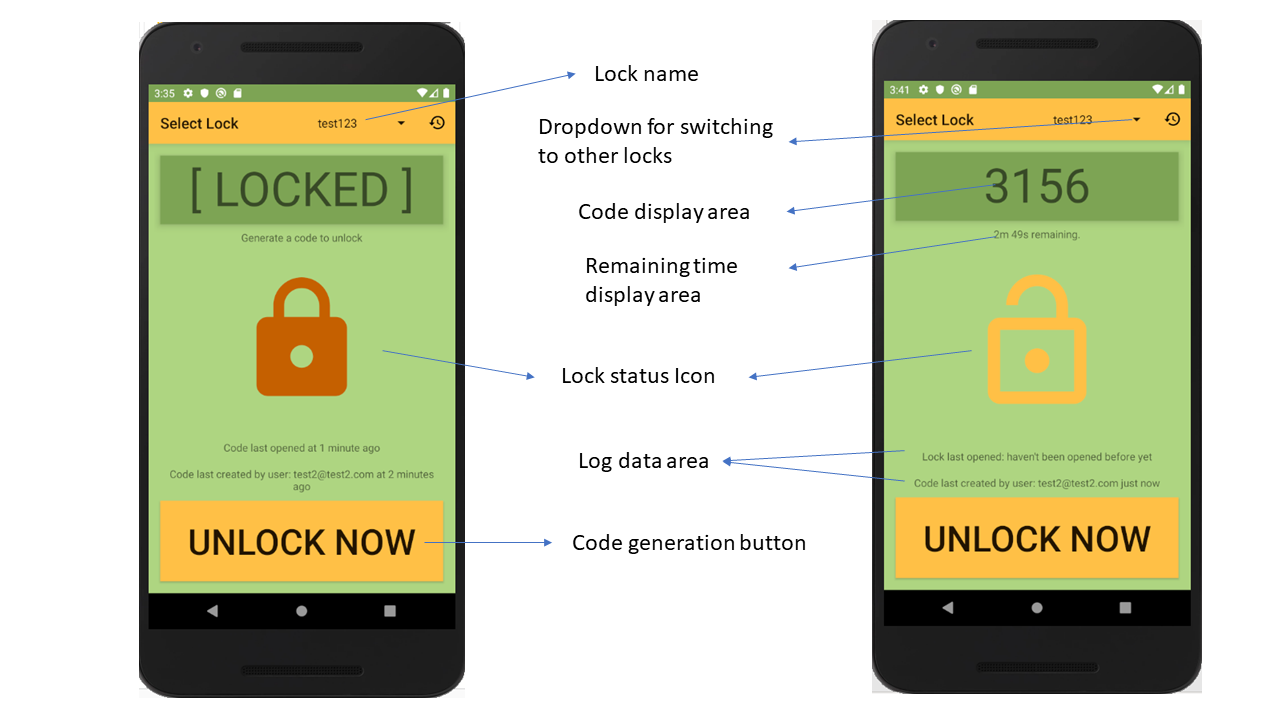
\includegraphics[width=\textwidth]{img/MainActivity.png}}
\caption{Main activity user interface of Android application}
\label{fig:mainActivity}
\end{figure*}

As you can see from this interface, users can easily switch to other locks by clicking the dropdown arrow. All lock names will be shown and the last row item is “Add new Lock” label where users can add a new lock by providing any necessary information to prove his or her ownership for the new lock. Once the user successfully added the new lock by clicking that item, its user-defined name will be shown in the dropdown. For the newly added lock, a closed lock icon is displayed to indicate there is not any valid code for this lock right now. Thus, users are expected to click the code generation button to generate a new code for the selected lock. Once the button is clicked, a dialogue will pop up to let the user pick the expiry date for the code, and the date picker is initiated to be one minute later than the current users’ local time by default. When users confirm the expiry date, the biometrics authentication will be triggered. Once users are authenticated, the new code generated by the server will be displayed to users in the code display area. And the remaining time label below will remind users how long this code remains valid. 




\section{Evaluation}
\subsection{Evaluation Methodology}
We perform usability studies to evaluate the usability of our system. First, three UBC undergraduates are invited to perform the study. They all have Computer Science or engineering related backgrounds and had experience of using normal keypad lock. They all learned sufficient knowledge about security and system design during their undergraduate study, which could give us more technical advice from a professional perspective.  A series of carefully designed tasks will be assigned to them, and after finishing the tasks, we will interview them individually to get some objective feedback for our smart lock prototype.

All tasks are designed to simulate the real user workflow in the real world. First, each user will download our Android application on their own Android phones (or we gave them a sample Android phone if they do not have one). Then, they will log in to our system using the test account we give to them. Second, after users have logged in, they are required to register the test lock using the lock information provided to them. In this process, users will figure out how to add locks in our Android application. Third, users are asked to generate the code for the test lock and using the code they generated to unlock the test lock, which is also the core functionalities of our prototype. We also repeated this task three times and recorded the time consumed to assess the speed properties of our system.  Finally, we let users generate a code with a short lifetime (e.g. one-minute expiry time) and unlock the lock once the code is expired. After this task, users will have a better understanding of how the design of the expiry time of our system works.

After users finished their tasks, several questions will be interviewed to them for assessing our system. First, we let the user rate our prototype in terms of ease of use on a scale of 1 to 10. Then, we asked them to compare and contrast our smart lock with traditional keypad lock.  Finally, users are asked to give constructive suggestions for our system.

\subsection{Study Results}
All three users successfully completed the tasks, although there were some small issues happened. User A had connection issues during login, but she succeeded in the second try. User C failed to unlock the lock using the generated code in the first time, the error response showed the code is expired, however, he tried to generate a new code and passed the authentication. User B did not have any issues and finished his tasks smoothly. The total time three users used to generate the code and unlock the door is shown in table~\ref{tab:time}.

\begin{table}[htbp]
\caption{Total time users consumed to unlock the lock}
\begin{center}
\begin{tabular}{|c|c|c|c|}
\hline
\textbf{User}&\textbf{A}&\textbf{B}&\textbf{C} \\
\hline
\textbf{1st Attempt} & \textbf{22s} & \textbf{20s} & \textbf{Failed (expired code)} \\
\hline
\textbf{2nd Attempt} & \textbf{17s} & \textbf{15s} & \textbf{19s} \\
\hline
\textbf{3rd Attempt} & \textbf{12s} & \textbf{13s} & \textbf{15s}  \\
\hline
\end{tabular}
\label{tab:time}
\end{center}
\end{table}
Regarding the first interviewed question, the results are shown in table~\ref{tab:rate}

\begin{table}[htbp]
\caption{Rates of overall usabilities given by three users}
\begin{center}
\begin{tabular}{|c|c|c|c|}
\hline
\textbf{User}&\textbf{A}&\textbf{B}&\textbf{C} \\
\hline
\textbf{Rate (out of 10)} & \textbf{8} & \textbf{7} & \textbf{7} \\
\hline
\end{tabular}
\label{tab:rate}
\end{center}
\end{table}
For the second question, user A believed she felt more secure when using our smart lock system since the code is one-time use with expiry time, while student B thought that although it is more secure than the traditional keypad lock, our system has reduced usability, because he only needs inputs four-digit number to unlock the door previously, whereas, he has to check his phone and use biometric to generate the code. User C has a similar opinion as user B and he also added that he will prefer to use traditional keypad lock unless our prototype has easier and simple user workflow.

For the third problem, both users A and C think setting expiry time for the code seems unnecessary and redundant, instead, they prefer a default expiry time. User B mentioned he wants to know who consumed the code to open the door other than when the code was used in log area of the main activity of the app.

\subsection{Discussion of the evaluation results}
Overall, the results show our prototype is still usable as the rate shown in table 2, two users give 7 out 10 while one user gave 8 points but this study also exposes many problems and limitations of our design. We will talk about the usability of our system according to five factors, speed, efficiency (Security mistake), learnability, memorability and user preference.
In terms of the speed properties, as the results listed from the table, users approximately cost 12-15 seconds on average to unlock. While the time length for authentication is not too long, it obviously reduces the speed properties compared with traditional keypad locks. However, some actions can be taken to accelerate this process. For instance, as suggested by user A and user C, we could remove the part of setting expiry time when users try to generate the code and using default expiry time instead. Meanwhile, we sacrificed the flexibility that users could set any expiry time they want.

The efficiency of our system is satisfying overall. All users did not get confused and make too many mistakes when they are performing the tasks, except some small issues do happen. Our Android application could be improved to provide a smoother user experience. For example, when once the user login, our Android app could remember the user’s identity so that users do not have to login again for a while. In addition, connection issues can be reduced by improving the performance of the server.

The learnability of our system can be demonstrated in table 1, as you can see users used less time to complete the authentication to unlock when they had a second or third attempt. This proved that our system is straightforward and easy to use, implying memorability also reach the standard. Users do not have to memorize anything except checking their phones to unlock the door.

Finally, regarding user preference, on the one hand, users believed our system does provide more security features, such as login, biometric authentication and one-time door code, etc. On the other hand, users complain about some other features. Other than the expiry time feature mentioned before, users like to see more traceable data such as those who unlock the door. However, this is a big challenge with our current design because it is hard to identify who unlock the door based on four random-generated digits he or she input but it is easier to tell the user when the lock was unlocked. Some of our members proposed to use four-digit number inserted before the actual code as user identity number. Nevertheless, it is a bad design since users need to remember and press more digits than before.


\section{Discussion}

\section{Conclusion}


\section*{References}

Please number citations consecutively within brackets \cite{b1}. The 
sentence punctuation follows the bracket \cite{b2}. Refer simply to the reference 
number, as in \cite{b3}---do not use ``Ref. \cite{b3}'' or ``reference \cite{b3}'' except at 
the beginning of a sentence: ``Reference \cite{b3} was the first $\ldots$''

Number footnotes separately in superscripts. Place the actual footnote at 
the bottom of the column in which it was cited. Do not put footnotes in the 
abstract or reference list. Use letters for table footnotes.

Unless there are six authors or more give all authors' names; do not use 
``et al.''. Papers that have not been published, even if they have been 
submitted for publication, should be cited as ``unpublished'' \cite{b4}. Papers 
that have been accepted for publication should be cited as ``in press'' \cite{b5}. 
Capitalize only the first word in a paper title, except for proper nouns and 
element symbols.

For papers published in translation journals, please give the English 
citation first, followed by the original foreign-language citation \cite{b6}.

\begin{thebibliography}{00}
\bibitem{JG}J. Golbeck, “Usable Security,” Open CSF: Open Computer Science Foundations, 01-Aug-2016. [Online]. Available: https://www.youtube.com/watch?v=O4QbOFDUVao. [Accessed: 04-Dec-2019].

\end{thebibliography}
\vspace{12pt}
\color{red}
IEEE conference templates contain guidance text for composing and formatting conference papers. Please ensure that all template text is removed from your conference paper prior to submission to the conference. Failure to remove the template text from your paper may result in your paper not being published.

\end{document}
